\section*{Appendix} 

Here are some of our results we did not further use in our report, because we did not investigate them.
However, these graphs may be really interesting to investigate further.\\
\\
First, we show our results on the effect of the Happiness Rule on the total number of moves.

\begin{figure}[H]
	\centering
    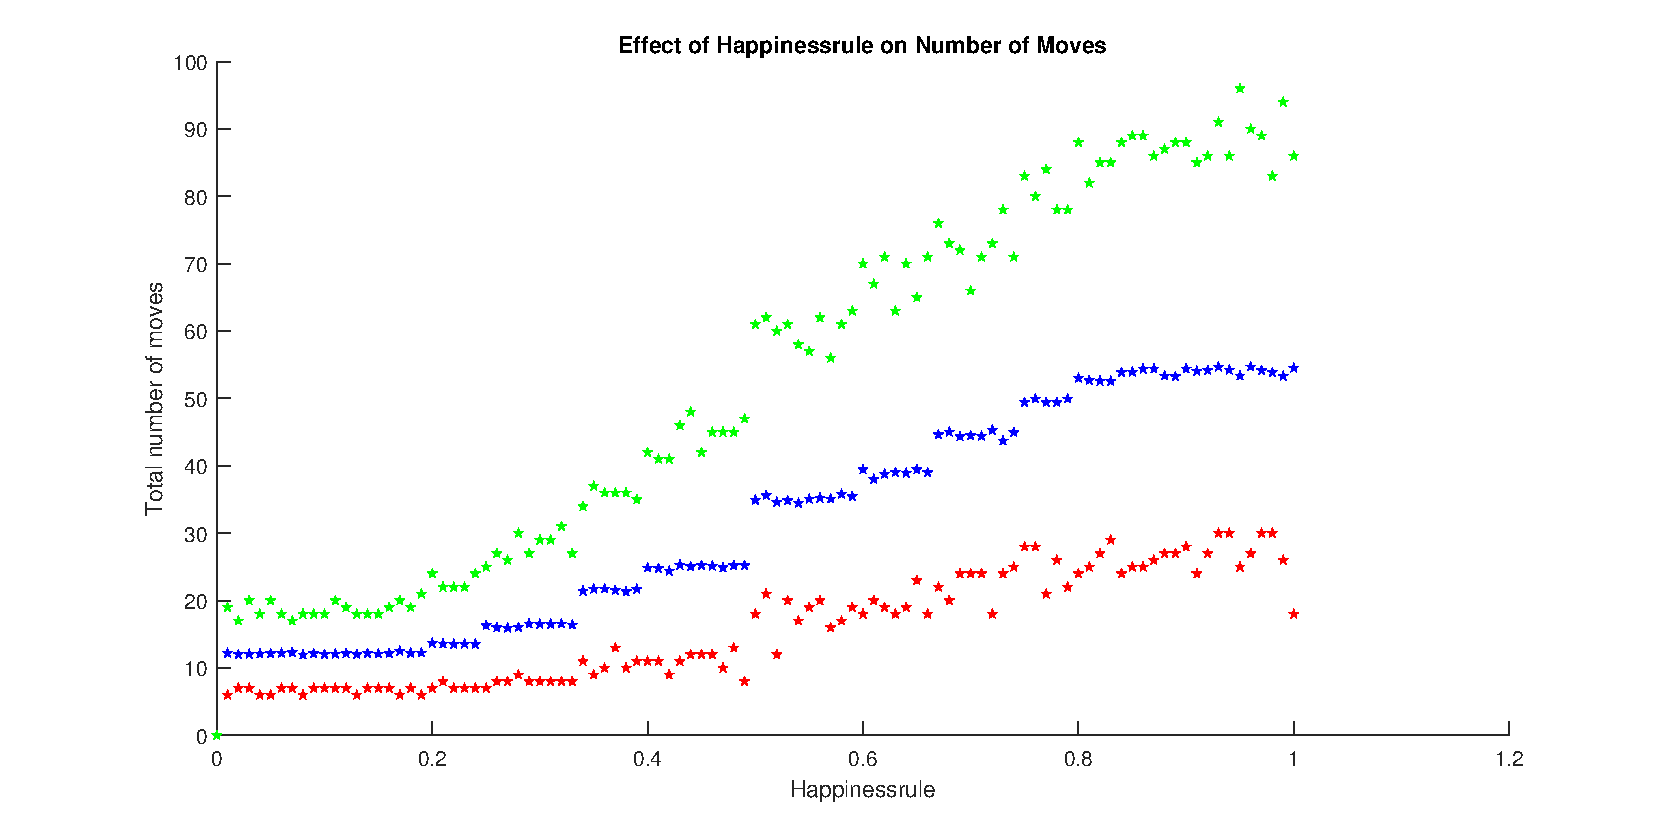
\includegraphics[width=\textwidth]{happinessregel-aantmov.pdf}
    \caption{Effect of the Happiness Rule on the total number of moves with the standard settings}
    \label{fig:happinessrule-moves}
\end{figure}

Figure \ref{fig:randmove-generations} shows the effect of the random move on the number of generations.

\begin{figure}[H]
	\centering
    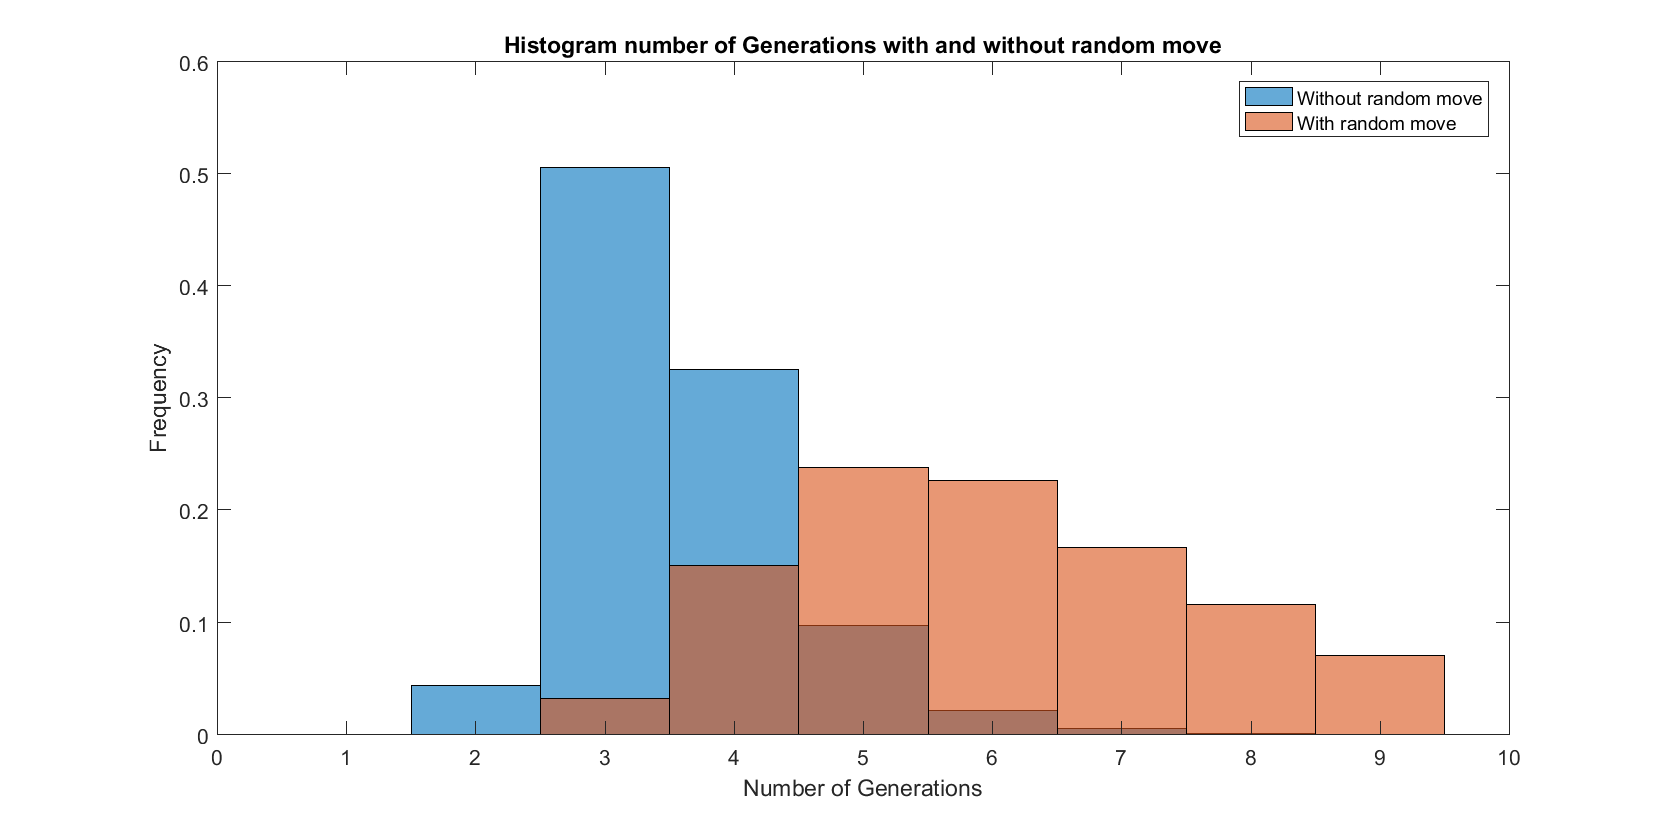
\includegraphics[width=\textwidth]{histaantgenrandverp.pdf}
    \caption{Effect of the random move on the number of generations with the standard settings}
    \label{fig:randmove-generations}
\end{figure}

Figure \ref{fig:nbho-generations} shows the effect of the order of neighbourhood on the number of generations, the number of moves, the segregration fraction and the average happiness of all individuals in equilibrium.

\begin{figure}[H]
	\centering
    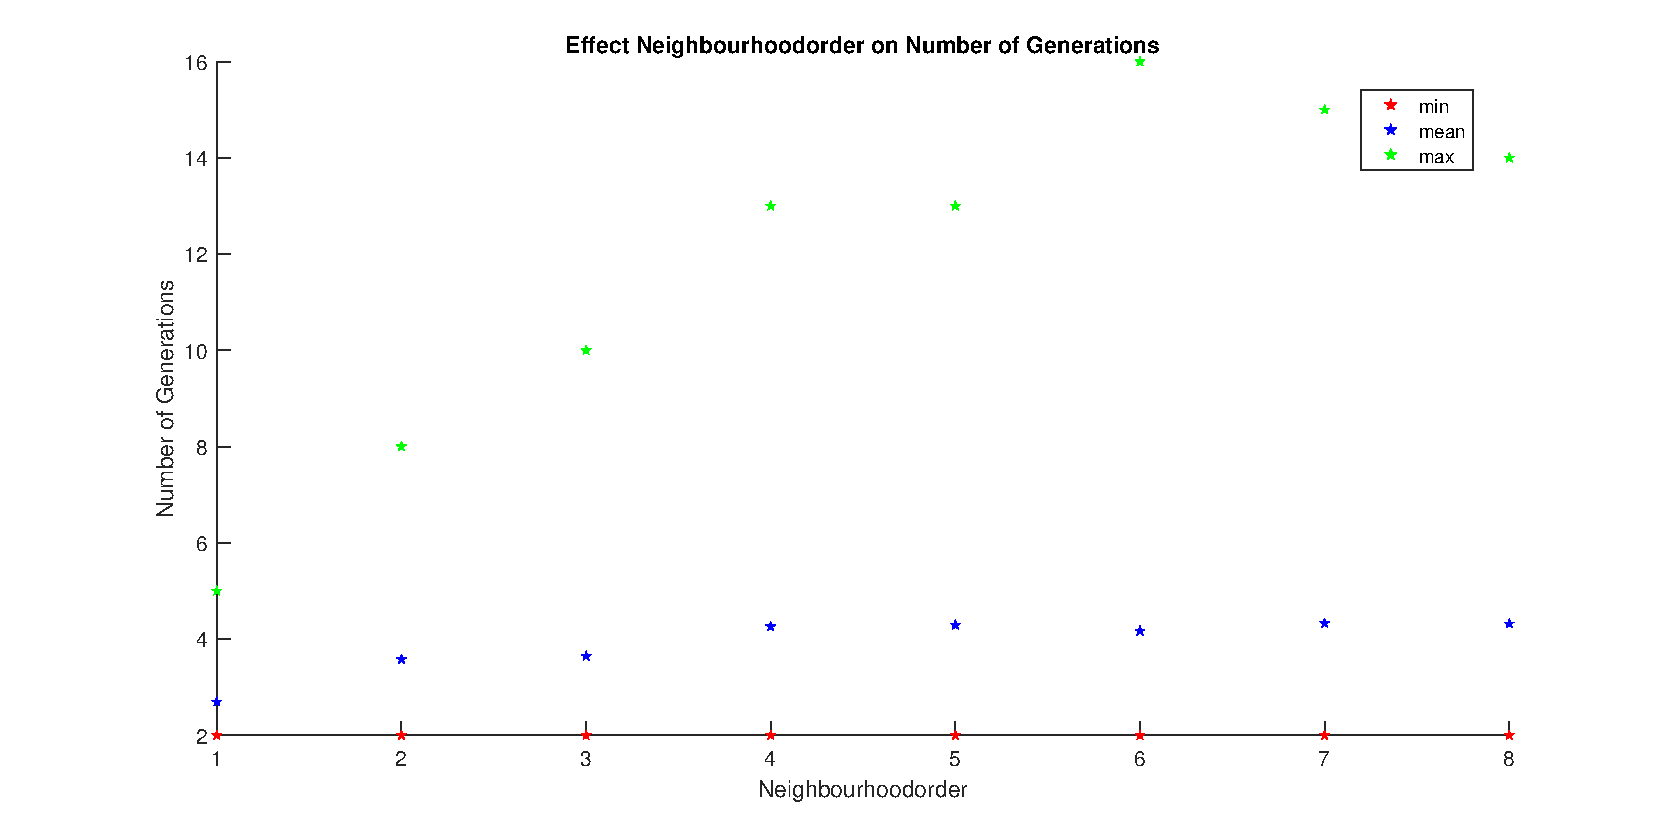
\includegraphics[width=\textwidth]{buurtorde-aantgen.pdf}
    \caption{Effect of the Neighbourhood order on the number of generations on the standard board}
    \label{fig:nbho-generations}
\end{figure}

\begin{figure}[H]
	\centering
    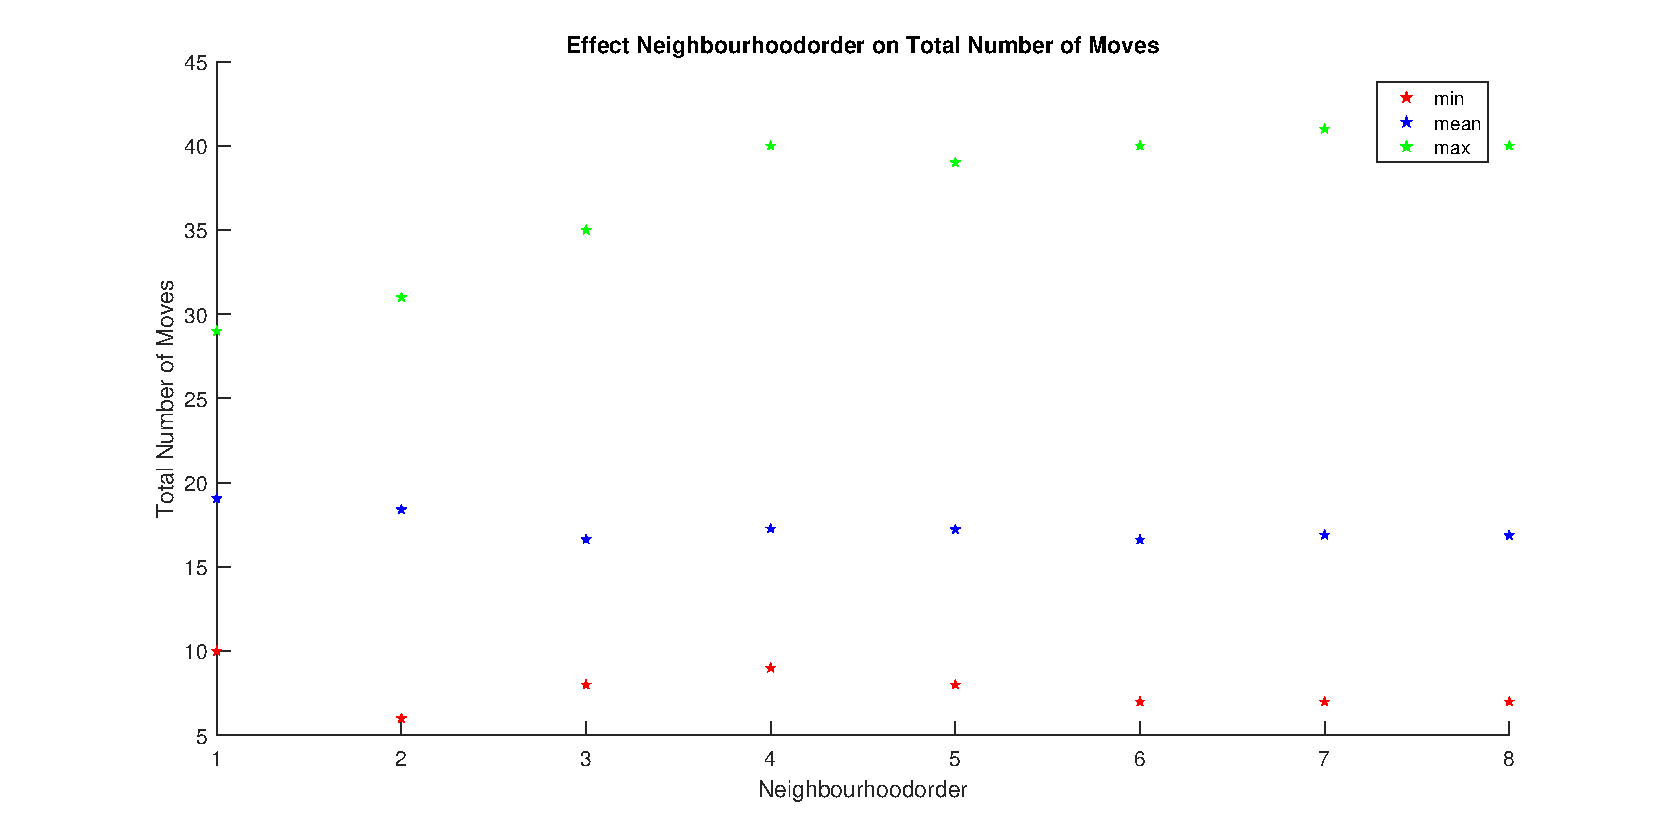
\includegraphics[width=\textwidth]{buurtorde-aantmov.pdf}
    \caption{Effect of the Neighbourhood order on the total number of moves on the standard board}
    \label{fig:nbho-moves}
\end{figure}

\begin{figure}[H]
	\centering
    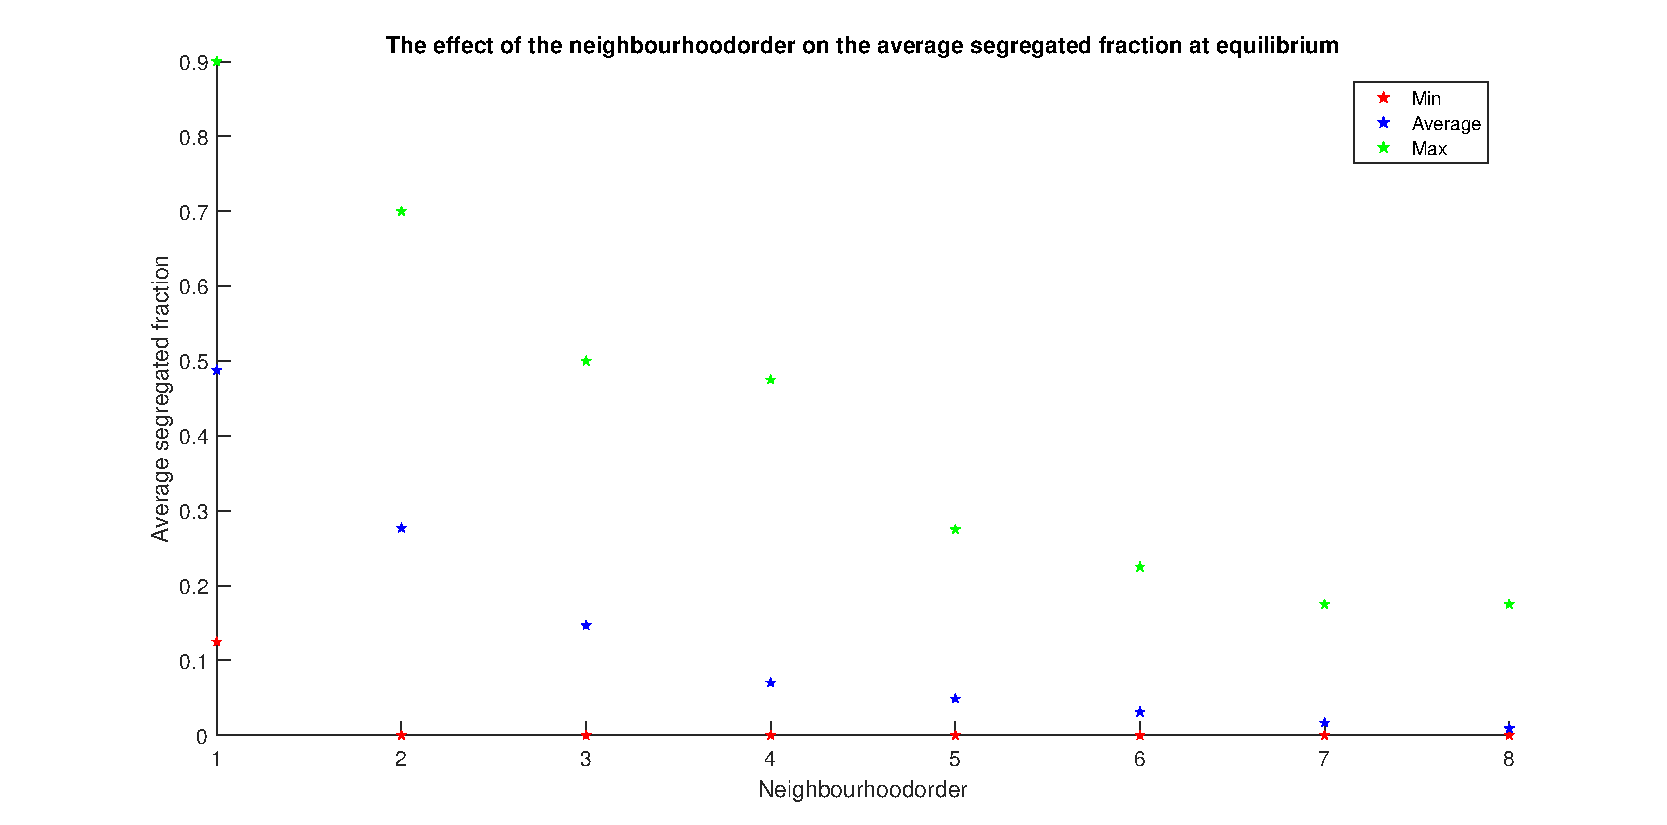
\includegraphics[width=\textwidth]{buurtorde-segreind.pdf}
    \caption{Effect of the Neighbourhood order on the segregated fraction in equilibrium on the standard board}
    \label{fig:nbho-segregation}
\end{figure}

\begin{figure}[H]
	\centering
    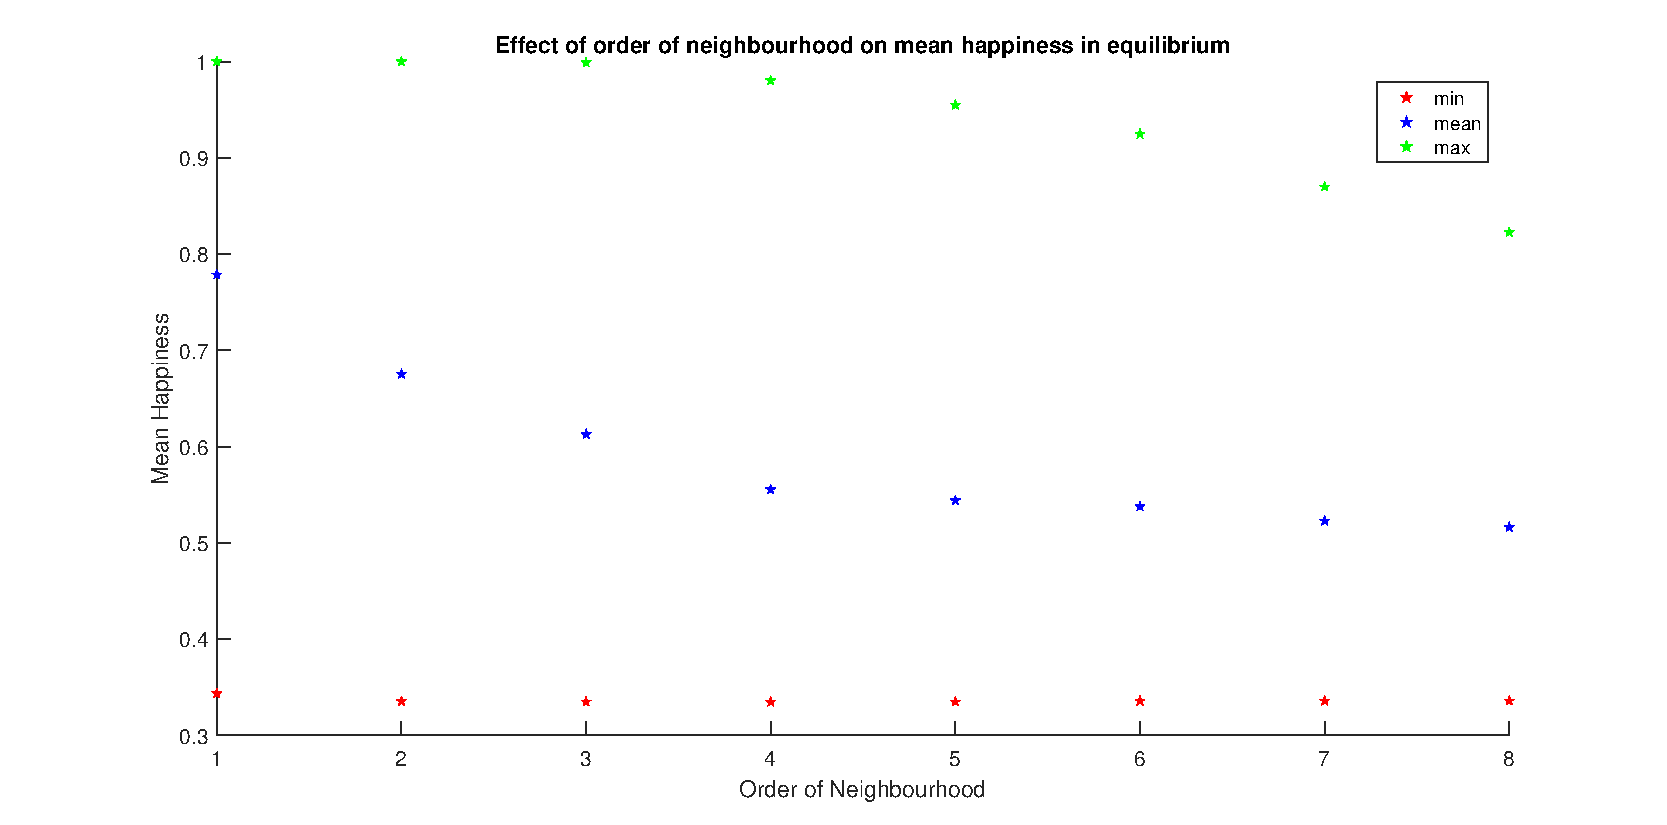
\includegraphics[width=\textwidth]{buurtorde-gemeindhappiness.pdf}
    \caption{Effect of the Neighbourhood order on the mean happiness in equilibrium on the standard board}
    \label{fig:nbho-happiness}
\end{figure}

Furhtermore, the effect of the criminals is really interesting. Figures \ref{fig:cr-aantgen} to \ref{fig:cr-segr} show the effects of the number of criminals on the standard board (The maximum number of criminals is $40$).

\begin{figure}[H]
	\centering
    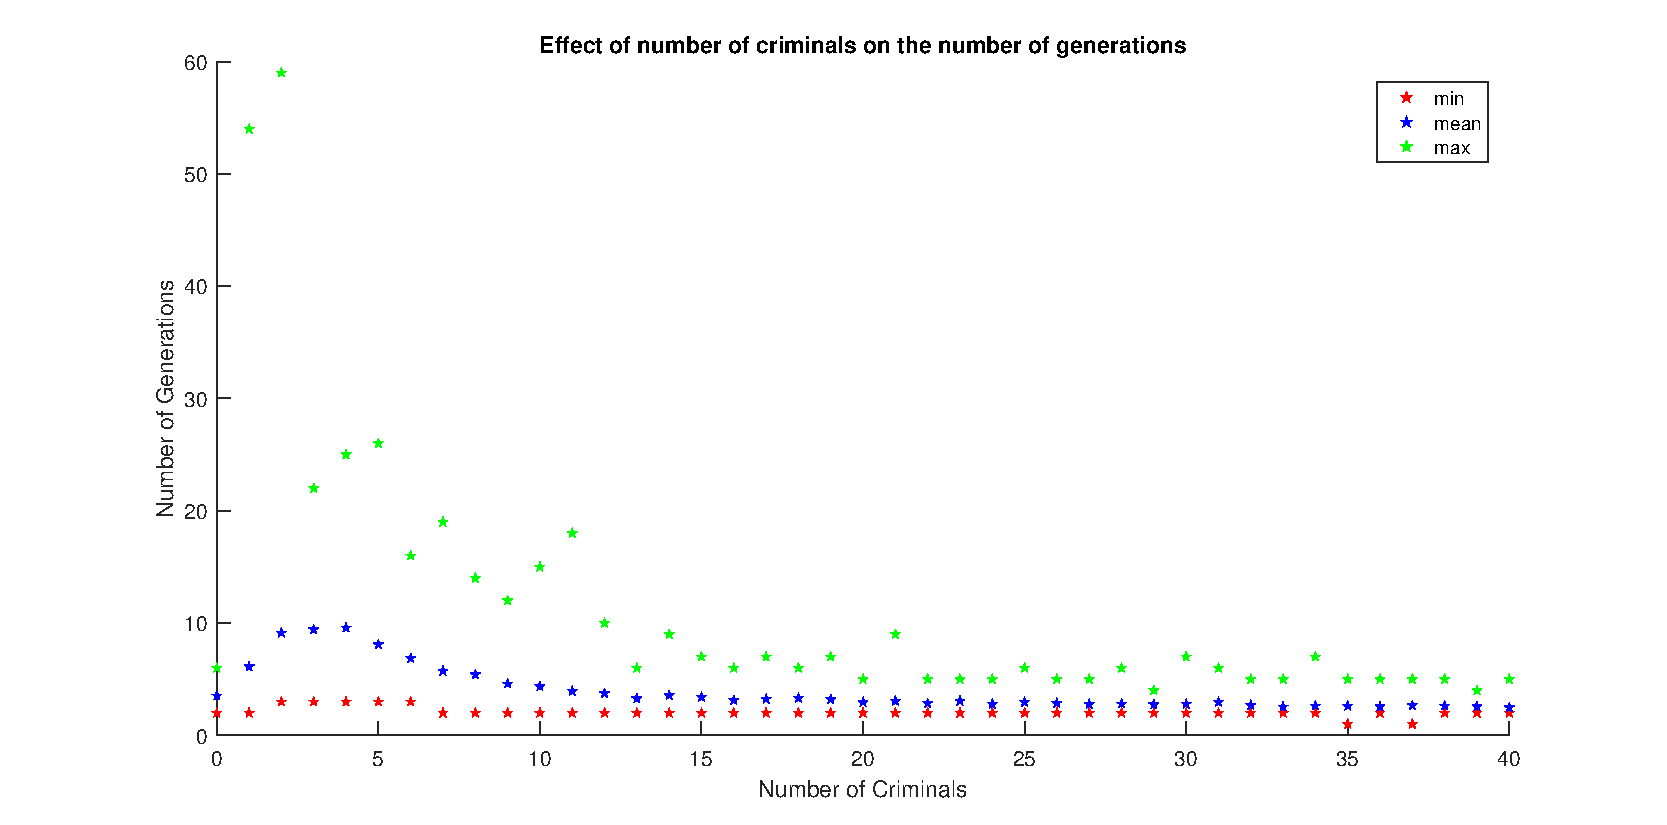
\includegraphics[width=\textwidth]{aantcrim-aantgen.pdf}
    \caption{Effect of the number of criminals on the number of generations on the standard board }
    \label{fig:cr-aantgen}
\end{figure}

\begin{figure}[H]
	\centering
    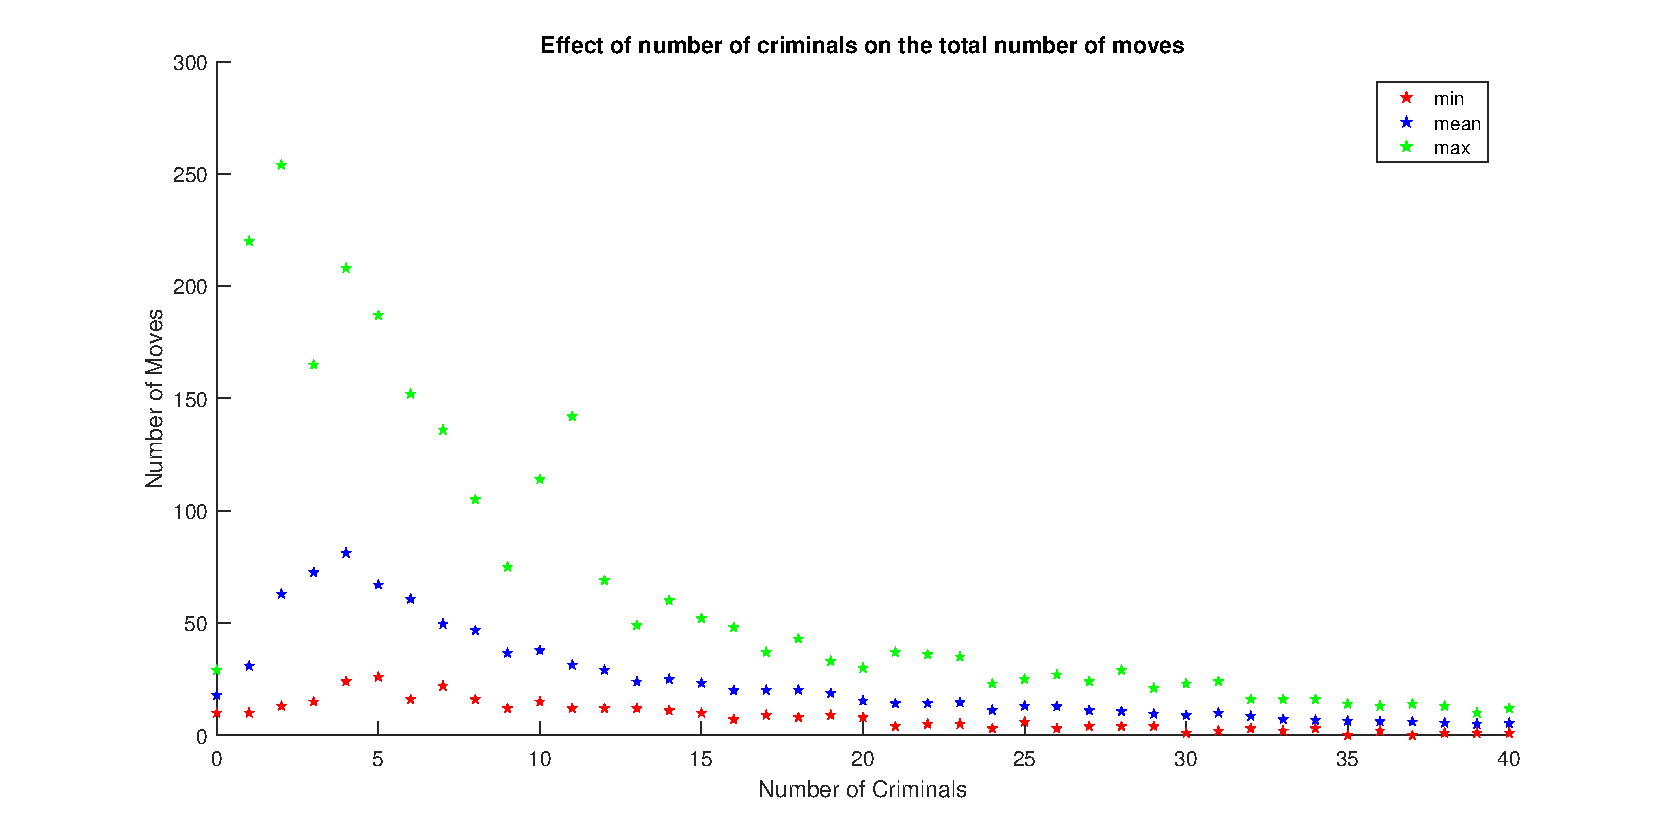
\includegraphics[width=\textwidth]{aantcrim-aantmov.pdf}
    \caption{Effect of the number of criminals on the total number of moves on the standard board}
    \label{fig:cr-aantmov}
\end{figure}

\begin{figure}[H]
	\centering
    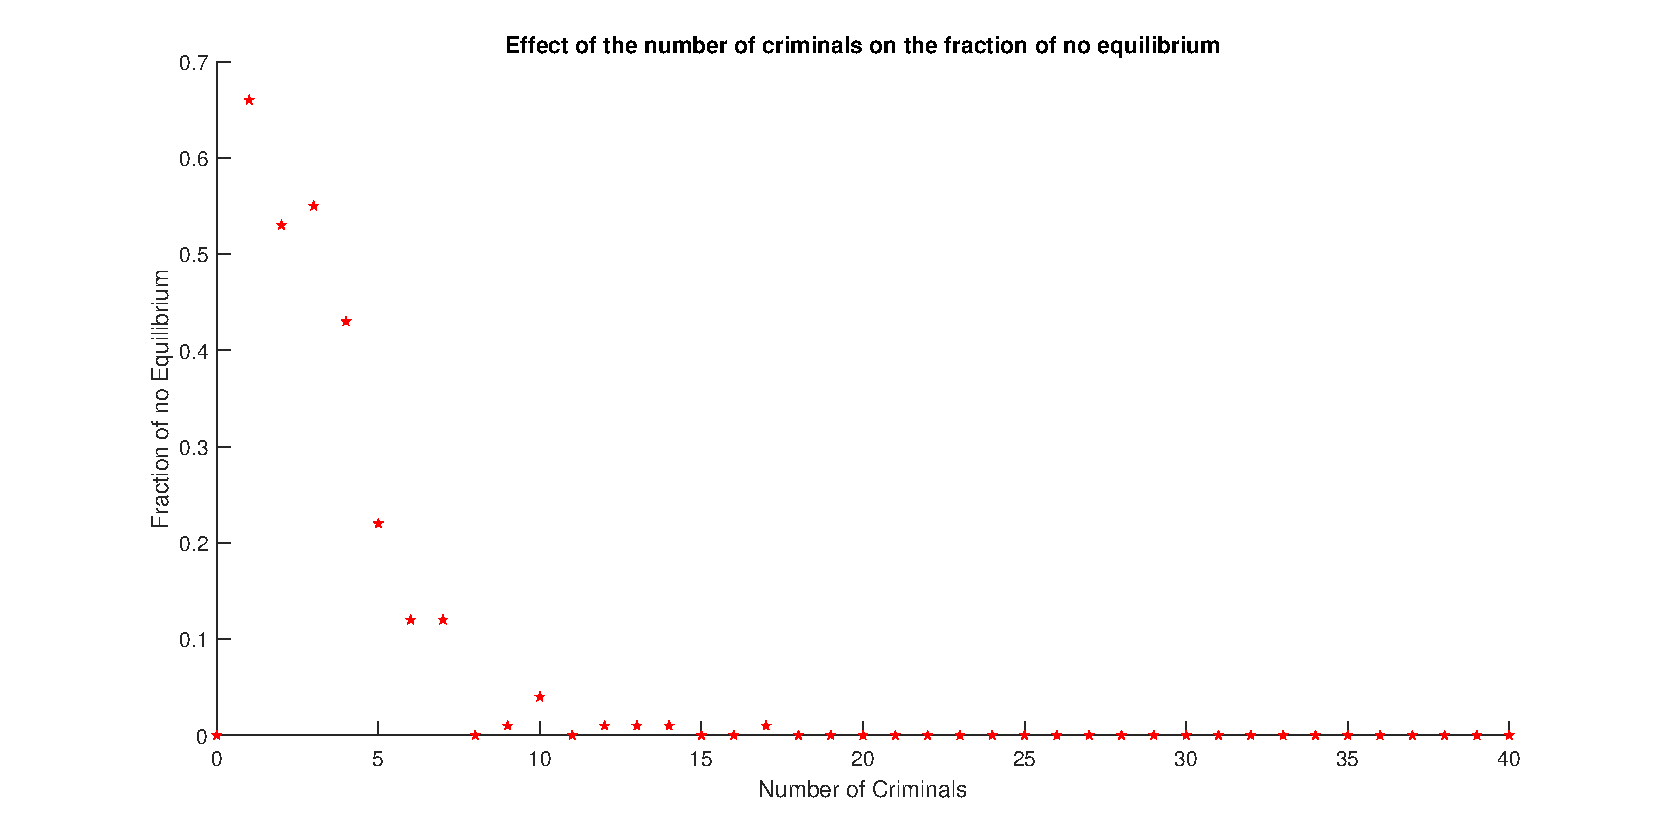
\includegraphics[width=\textwidth]{aantcrim-fracnoeq.pdf}
    \caption{Effect of the number of criminals on the relative number of times with no equilibrium on the standard board}
    \label{fig:cr-noeq}
\end{figure}

\begin{figure}[H]
	\centering
    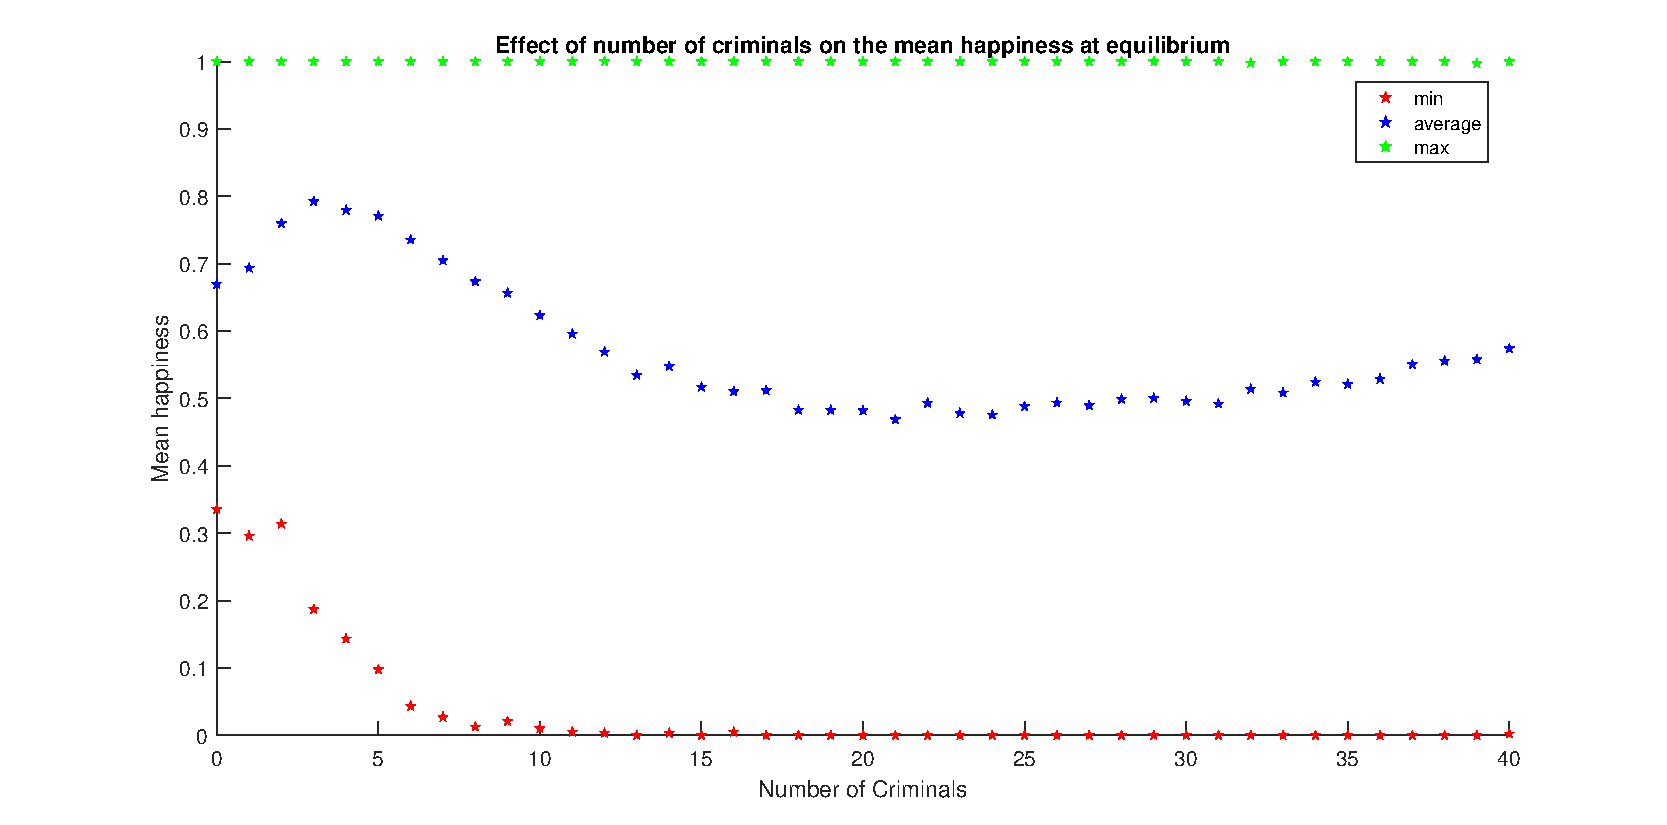
\includegraphics[width=\textwidth]{aantcrim-gemeindhappiness.pdf}
    \caption{Effect of the number of criminals on the mean happiness at equilibrium on the standard board}
    \label{fig:cr-happ}
\end{figure}

\begin{figure}[H]
	\centering
    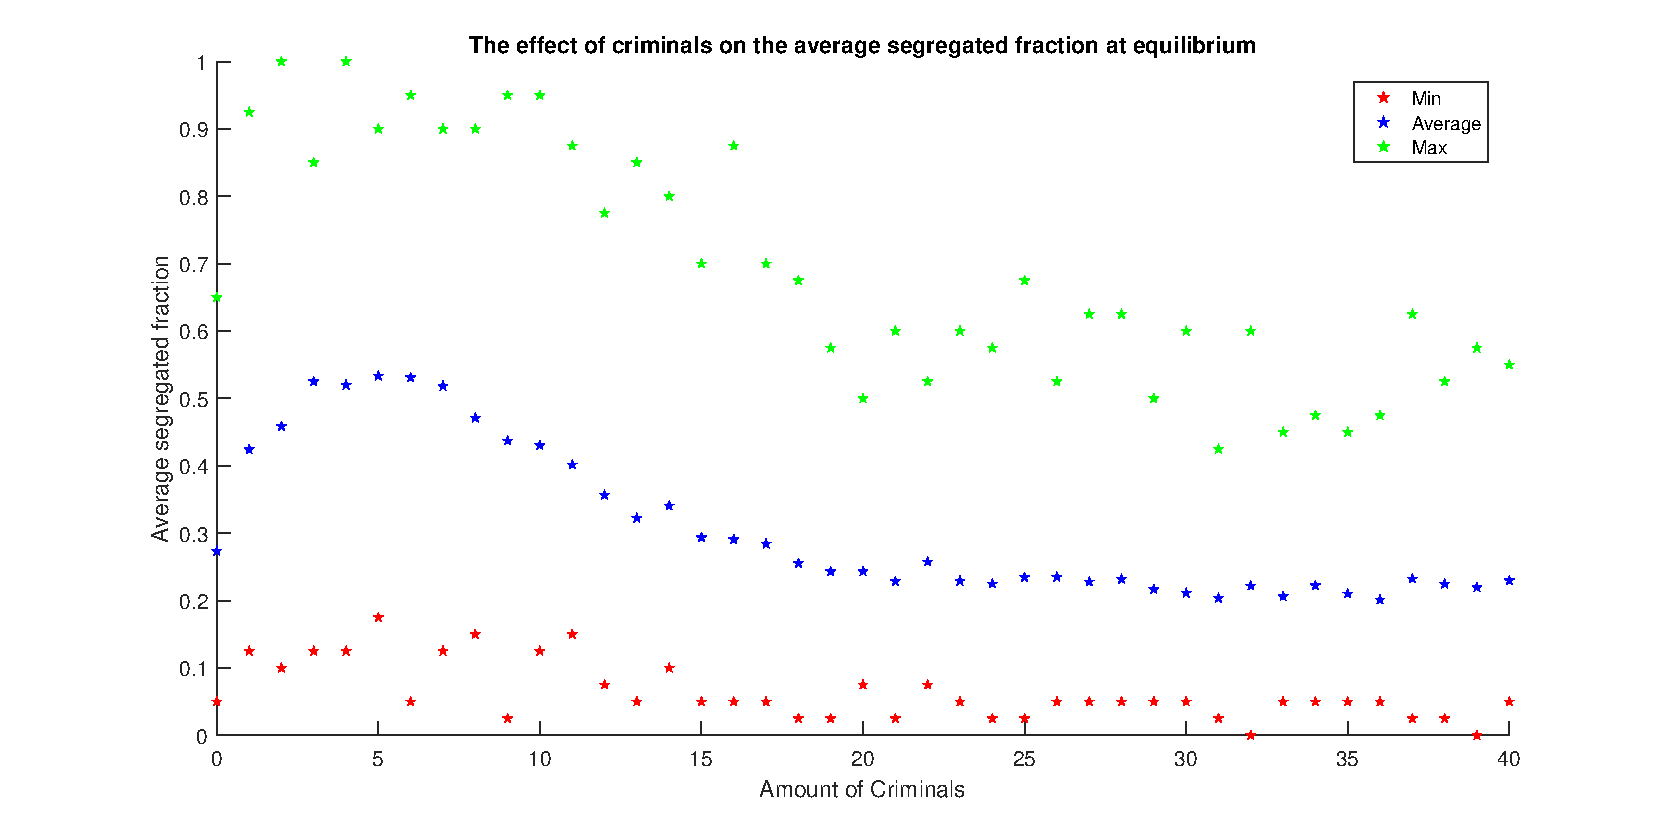
\includegraphics[width=\textwidth]{aantcrim-segreind.pdf}
    \caption{Effect of the number of criminals on the mean segregation on the standard board}
    \label{fig:cr-segr}
\end{figure}

